%%%%%%%%%%%%%%%%%%%%%%%%%%%%%%%%%%%%%%%%%
% Short Sectioned Assignment
% LaTeX Template
% Version 1.0 (5/5/12)
%
% This template has been downloaded from:
% http://www.LaTeXTemplates.com
%
% Original author:
% Frits Wenneker (http://www.howtotex.com)
%
% License:
% CC BY-NC-SA 3.0 (http://creativecommons.org/licenses/by-nc-sa/3.0/)
%
%%%%%%%%%%%%%%%%%%%%%%%%%%%%%%%%%%%%%%%%%

%----------------------------------------------------------------------------------------
%	PACKAGES AND OTHER DOCUMENT CONFIGURATIONS
%----------------------------------------------------------------------------------------

\documentclass[paper=a4, fontsize=11pt]{scrartcl} % A4 paper and 11pt font size

\usepackage[T1]{fontenc} % Use 8-bit encoding that has 256 glyphs
%\usepackage{fourier} % Use the Adobe Utopia font for the document - comment this line to return to the LaTeX default
\usepackage[english]{babel} % English language/hyphenation
\usepackage[utf8]{inputenc}  %allows non-English characters
\usepackage{amsmath,amsfonts,amsthm} % Math packages
\usepackage{float}

\usepackage{sectsty} % Allows customizing section commands
%\allsectionsfont{\centering \normalfont\scshape} % Make all sections centered, the default font and small caps
\allsectionsfont{\centering}

\usepackage{fancyhdr} % Custom headers and footers
\pagestyle{fancyplain} % Makes all pages in the document conform to the custom headers and footers
\fancyhead{} % No page header - if you want one, create it in the same way as the footers below
\fancyfoot[L]{} % Empty left footer
\fancyfoot[C]{} % Empty center footer
\fancyfoot[R]{\thepage} % Page numbering for right footer
\renewcommand{\headrulewidth}{0pt} % Remove header underlines
\renewcommand{\footrulewidth}{0pt} % Remove footer underlines
\setlength{\headheight}{13.6pt} % Customize the height of the header

%\usepackage{geometry}
%\usepackage{pdflscape}


%\numberwithin{equation}{section} % Number equations within sections (i.e. 1.1, 1.2, 2.1, 2.2 instead of 1, 2, 3, 4)
%\numberwithin{figure}{section} % Number figures within sections (i.e. 1.1, 1.2, 2.1, 2.2 instead of 1, 2, 3, 4)
%\numberwithin{table}{section} % Number tables within sections (i.e. 1.1, 1.2, 2.1, 2.2 instead of 1, 2, 3, 4)

%\setlength\parindent{0pt} % Removes all indentation from paragraphs - comment this line for an assignment with lots of text

\usepackage{caption}
%\usepackage{topcapt}

\usepackage{booktabs}

\usepackage{graphicx}
\usepackage{adjustbox}
\graphicspath{{../data/}}


%shortcuts for typing variance and expectation
\newcommand{\E}{\mathrm{E}}
\newcommand{\Var}{\mathrm{Var}}

%----------------------------------------------------------------------------------------
%	TITLE SECTION
%----------------------------------------------------------------------------------------

\newcommand{\horrule}[1]{\rule{\linewidth}{#1}} % Create horizontal rule command with 1 argument of height

\title{
\normalfont \normalsize
\textsc{UPC - Complex and Social Networks} \\ [25pt] % Your university, school and/or department name(s)
\horrule{0.5pt} \\[0.4cm] % Thin top horizontal rule
\huge Lab5: Finding community structures \\ % The assignment title
\horrule{2pt} \\[0.5cm] % Thick bottom horizontal rule
}

\author{Jakub Šalagovič\\Simon Van den Eynde} % Your name

\date{\normalsize\today} % Today's date or a custom date

\begin{document}


\maketitle % Print the title


%----------------------------------------------------------------------------------------
%	INTRO
%----------------------------------------------------------------------------------------

\section{Introduction}
This report consists of $2$ parts. In the first part we will compare some of igraph's community-finding algorithms on specifically chosen graphs, using the metrics: Triangle Partition Ratio (high is best), expansion (low is best), conductance (low is best) and modularity (high is best). In the second part we will analyse if it makes sense to use fast-greedy community detection algorithm of provided Wikipedia network. 
\section{Task 1 -- Comparison of community-finding algorithms}
\subsection{Results}
% latex table generated in R 3.1.2 by xtable 1.8-2 package
% Wed Nov 23 21:28:34 2016
\begin{table}[ht]
\centering
\begin{tabular}{rrrrr}
  \hline
 & TPT & expansion & conductance & modularity \\ 
  \hline
edge.betweenness & 1.000 & 4.400 & 0.524 & 0.425 \\ 
  
             fastgreedy & 1.000 & 4.400 & 0.524 & 0.425 \\ 
  
             label.propagation & 1.000 & 4.160 & 0.482 & 0.340 \\ 
  
             leading.eigenvector & 1.000 & 3.200 & 0.333 & 0.000 \\ 
  
             multilevel & 1.000 & 4.400 & 0.524 & 0.425 \\ 
  
             optimal & 1.000 & 4.400 & 0.524 & 0.425 \\ 
  
             spinglass & 1.000 & 4.400 & 0.524 & 0.425 \\ 
  
             walktrap & 1.000 & 4.400 & 0.524 & 0.425 \\ 
  
             infomap & 1.000 & 4.400 & 0.524 & 0.425 \\ 
   \hline
\end{tabular}
\caption{Metrics for HanoiTower(5,2) (HT)} 
\end{table}
% latex table generated in R 3.1.2 by xtable 1.8-2 package
% Wed Nov 23 21:28:34 2016
\begin{table}[ht]
\centering
\begin{tabular}{rrrrr}
  \hline
 & TPT & expansion & conductance & modularity \\ 
  \hline
edge.betweenness & 0.000 & 1.933 & 0.476 & 0.451 \\ 
  
             fastgreedy & 0.000 & 2.000 & 0.501 & 0.411 \\ 
  
             label.propagation & 0.000 & 1.800 & 0.430 & 0.420 \\ 
  
             leading.eigenvector & 0.000 & 1.667 & 0.385 & 0.389 \\ 
  
             multilevel & 0.000 & 1.933 & 0.476 & 0.451 \\ 
  
             optimal & 0.000 & 1.933 & 0.476 & 0.451 \\ 
  
             spinglass & 0.000 & 2.067 & 0.527 & 0.442 \\ 
  
             walktrap & 0.000 & 1.933 & 0.476 & 0.451 \\ 
  
             infomap & 0.000 & 1.867 & 0.456 & 0.416 \\ 
   \hline
\end{tabular}
\caption{Metrics for Double Star Snark (DSS)} 
\end{table}
% latex table generated in R 3.1.2 by xtable 1.8-2 package
% Wed Nov 23 21:28:34 2016
\begin{table}[ht]
\centering
\begin{tabular}{rrrrr}
  \hline
 & TPT & expansion & conductance & modularity \\ 
  \hline
edge.betweenness & 0.600 & 2.467 & 0.529 & 0.228 \\ 
  
             fastgreedy & 0.400 & 2.733 & 0.609 & 0.217 \\ 
  
             label.propagation & 1.000 & 1.800 & 0.333 & 0.000 \\ 
  
             leading.eigenvector & 1.000 & 1.800 & 0.333 & 0.000 \\ 
  
             multilevel & 0.600 & 2.600 & 0.565 & 0.222 \\ 
  
             optimal & 0.600 & 2.467 & 0.530 & 0.239 \\ 
  
             spinglass & 0.400 & 2.600 & 0.577 & 0.230 \\ 
  
             walktrap & 0.400 & 2.600 & 0.575 & 0.181 \\ 
  
             infomap & 1.000 & 1.800 & 0.333 & 0.000 \\ 
   \hline
\end{tabular}
\caption{Metrics for the Dorovtsev-Goltsev-Mendes(3) Graph (DGM)} 
\end{table}
% latex table generated in R 3.1.2 by xtable 1.8-2 package
% Wed Nov 23 21:28:35 2016
\begin{table}[ht]
\centering
\begin{tabular}{rrrrr}
  \hline
 & TPT & expansion & conductance & modularity \\ 
  \hline
edge.betweenness & 0.000 & 1.075 & 0.381 & 0.680 \\ 
  
             fastgreedy & 0.000 & 1.100 & 0.393 & 0.678 \\ 
  
             label.propagation & 0.000 & 1.200 & 0.451 & 0.614 \\ 
  
             leading.eigenvector & 0.000 & 1.075 & 0.381 & 0.680 \\ 
  
             multilevel & 0.000 & 1.100 & 0.393 & 0.678 \\ 
  
             optimal & 0.000 & 1.075 & 0.381 & 0.680 \\ 
  
             spinglass & 0.000 & 1.100 & 0.393 & 0.678 \\ 
  
             walktrap & 0.000 & 1.125 & 0.406 & 0.652 \\ 
  
             infomap & 0.000 & 1.125 & 0.406 & 0.670 \\ 
   \hline
\end{tabular}
\caption{Metrics for Barabasi-Albert (BA)} 
\end{table}
% latex table generated in R 3.1.2 by xtable 1.8-2 package
% Wed Nov 23 21:28:35 2016
\begin{table}[ht]
\centering
\begin{tabular}{rrrrr}
  \hline
 & TPT & expansion & conductance & modularity \\ 
  \hline
edge.betweenness & 0.794 & 3.000 & 0.497 & 0.401 \\ 
  
             fastgreedy & 0.824 & 2.853 & 0.454 & 0.381 \\ 
  
             label.propagation & 0.882 & 2.706 & 0.427 & 0.338 \\ 
  
             leading.eigenvector & 0.735 & 3.059 & 0.502 & 0.393 \\ 
  
             multilevel & 0.794 & 2.912 & 0.468 & 0.419 \\ 
  
             optimal & 0.794 & 2.912 & 0.468 & 0.420 \\ 
  
             spinglass & 0.794 & 2.912 & 0.468 & 0.420 \\ 
  
             walktrap & 0.588 & 3.235 & 0.545 & 0.353 \\ 
  
             infomap & 0.882 & 2.706 & 0.419 & 0.402 \\ 
   \hline
\end{tabular}
\caption{Metrics for Zachary's Karate network (ZK)} 
\end{table}

\newpage

\subsection{Discussion}
For more information on the chosen graphs, see section \ref{meth}. 
\begin{itemize}
\item In general we notice that the modularity sometimes becomes zero, this happens only if the entire network is one community. In this case we can discard these findings.
\item In graphs without triangles (BA, DSS) or with many triangles (HT) we find that that the Triangle Partition Ratio does not convey any useful information.
\item We see that for if there are clear communities as in HT, almost every community-finding method can identify them correctly.
\item When looking at the metric values for the DSS network, we see that the leading.eigenvalue gives rise a special community structure. Its expansion and conductance are a lot lower than for other graphs, which is good. But its modularity is also a lot lower, which is a bad sign. When comparing network sizes (not included) we note it is the only community structure which consists of only $2$ communities. So depending on how many communities you want, you might consider using different metrics our different community-finding methods.
\item The values for the conductance and expansion of the BA network are lower than that of other networks. Also the modularity is higher. This means that this power-law delivers stronger communities than many other graphs.
\end{itemize}


\subsection{Methods}\label{meth}
\subsection{Graphs}
We chose 5 different graphs. As a real network we chose Zachary's karate (ZK) network. We also analysed a Barab\'{a}si-Albert (BA) graph on $40$ vertices.
Furthermore we considered $3$ special graphs:
\paragraph{HanoiTower(5,2) (HT)}
This graph has as nodes the game states of Hanoi Tower game with $5$ pegs and $2$ disks, there is an edge if you can go from one game state to another in one move. This graph basically consists of $5$ copies of $K_{5}$ which are sparsely connected. See figure~\ref{ht}.
\paragraph{Double Star Snark (DSS)} This is graph is snark, which means it doesn't contain any triangle (this graph does only contain cycles with length $>5$), it is also cubic and has no bridges. It consists of $30$ vertices. See figure~\ref{dss}.
\paragraph{Dorovstev-Goltsev-Mendes graph (DGM)} This is a graph which can be constructed, starting with $K_{2}$, as follows: for every edge a triangle (add a vertex and 2 edges). If we do this $3$ times we get a graph with $15$ vertices, $27$ edges and a lot of triangles. See figure~\ref{dgm}.

%\paragraph{Randomization}
%For the standard graphs we chose (Hanoi Tower, double star snark and the Dorovstev-Goltsev-Mendes graph), we got counterintuitive results for our metrics. Because these graphs have many automorfisms and this is not so realistic, we randomised these networks. To do so, we rewired $15\%$ of all edges of these graphs.

\begin{figure}[htbp]
   \centering
   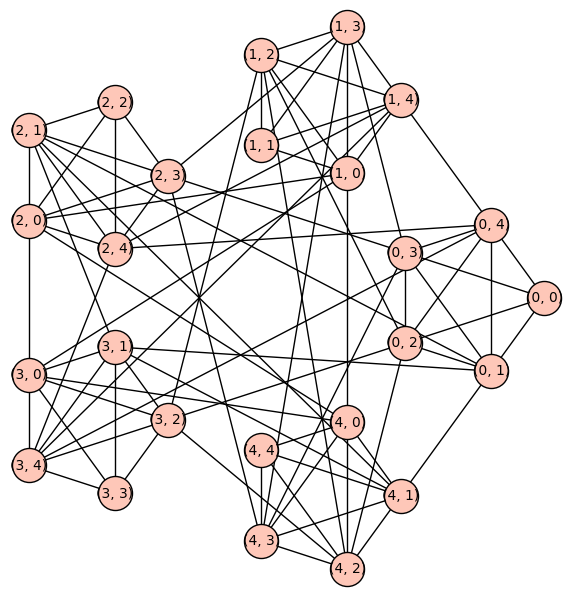
\includegraphics{ht} % requires the graphicx package
   \caption{The Hanoi Tower graph with $5$ pegs and $2$ discs. The labels on the vertices indicate the positions of the two discs ($(1,3)$ means: peg $1$ on disk $1$, peg $2$ on disc $2$)}
   \label{ht}
\end{figure}
\begin{figure}[htbp]
   \centering
   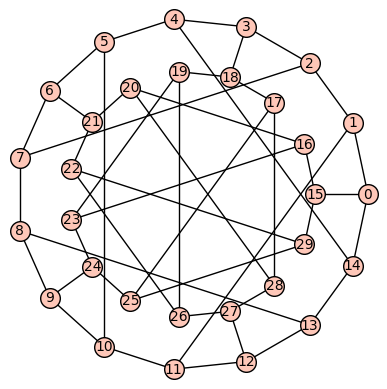
\includegraphics{dss} % requires the graphicx package
   \caption{The double star snark}
   \label{dss}
\end{figure}

\begin{figure}[htbp]
   \centering
   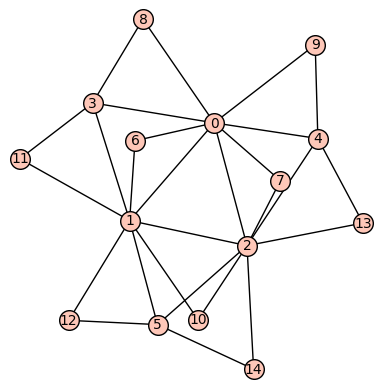
\includegraphics{dgm} % requires the graphicx package
   \caption{The Dorovstev-Goltsev-Mendes graph after $3$ iterations}
   \label{dgm}
\end{figure}

\section{Task 2 - Wikipedia}

For the task the we have chosen to use fast-greedy algorithm for community detection of this given network. Then we computed metrics discussed in the previous part, the results are as follows: modularity = $0.745$, expansion = $2.9$, conductance = $0.368$, TPR = $0.46$ (all values have been rounded to three decimal places). We can argue that modularity in this case is relatively high, which points to good division into communities. On the other hand, we have $2.9$ edges per node leaving community which can be either high or normal value for good division. It depends on a lot of factors, for example average number of edges per node and so on. Conductance, which is fraction of total edge volume that points outside community, with value $0.368$ can be higher that one expect for good division into communities, but it still does not mean the division into communities is not good. The same situation is also with triangle partition ratio.

Therefore we have needed to look if the dividing into communities make sense by different way. We have used three different approaches, each of them is presented below.

\subsection{Titles of each community}
The first approach is to look at titles (vertices) in communities and decide if it make sense to have them in one community (if we can find some common topic of other connection by meaning by titles in one community). Note that for this type of analysis one need to have some background knowledge in analysed terms. Therefore we skipped cases with terms we were not familiar with and for examples stated in this text we have selected the simple ones. Also it is impossible to manually analyse all communities, so we decided to look just for biggest and analyse first $n$ titles. The result for communities containing at least 50 titles can be found in the file \textit{WikiTitleCommunities.txt} attached to this document. 

For better visualisation and getting general view we decided to plot these results as text clouds. Every text cloud contains 50 selected titles from communities that contain at least 50 titles. The size of each title depends on the number of vertices the corresponding vertex is connected to. The text cloud for sample of 50 titles of the biggest community is displayed in the Fig.~\ref{TextCloud1}. We can say that almost all titles seems to be more or less related. Generally speaking, it looks like for each of the plotted text clouds we can find common topic or category to which they belong. All word clouds can be found in file \textit{WikiTextClouds.pdf} attached to this document.

\begin{figure}[H]
	\centering
	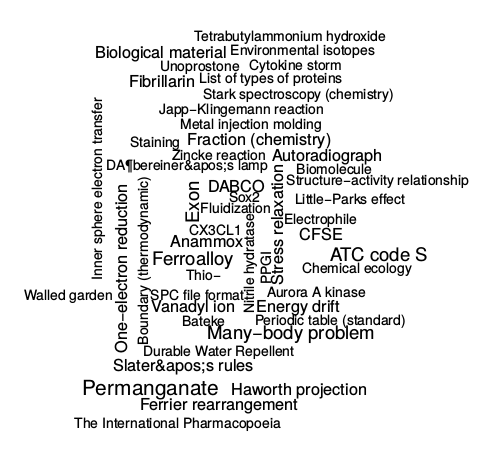
\includegraphics[scale=0.75,keepaspectratio]{TextCloud1}
	\caption{Text cloud of sample of 50 titles of Community 1}
	\label{TextCloud1}
\end{figure}

It is normal that there are cases when some titles looks completely unrelated to community they were assigned to. For example in Fig.~\ref{TextCloud8} we can see that titles look to be number related. But for example titles \textit{French punk} and \textit{Statue of Liberty Bike} clearly does not belongs to this category. Therefore we explored this whole community and have found that apart the \textit{number-related} articles there are smaller group of \textit{motorbike} and \textit{punk} related articles. It is normal that we do not get perfect communities, but results looks that in general make some sense. Apart the algorithm one can also question connections made by authors and editors of articles.
\begin{figure}[H]
	\centering
	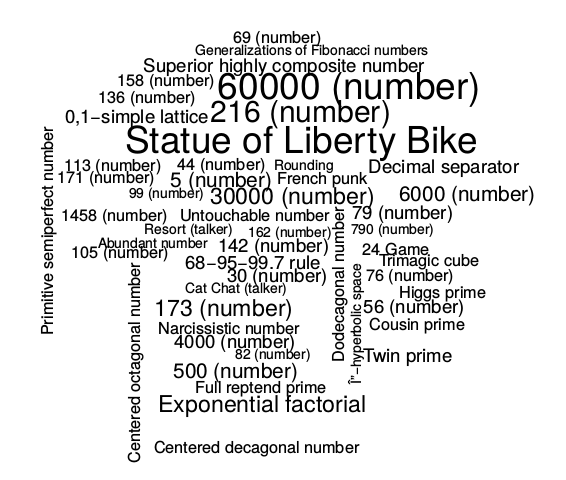
\includegraphics[scale=0.75,keepaspectratio]{TextCloud8}
	\caption{Text cloud of sample of 50 titles of Community 8}
	\label{TextCloud8}
\end{figure}

\subsection{Membership of neighbours}
The next approach is to look at the all neighbours of selected vertex and analyse if all of them are in community that makes sense regarding to the selected vertex and his community. For each vertex we plotted this sub-graph displaying corresponding communities in one figure. To make it easy to analyse we decided to use star layout with the corresponding vertex in the middle and its neighbours around. For the reasons mentioned earlier it is impossible to analyse results for all vertices, so we decided to plot just vertices that has 20 neighbours. The 20 neighbours are value large enough to find some general behaviour but it is still easy to visualise and analyse. All graphs for vertices with number of neighbours equal to 20 can be found in file \textit{WikiNeighboursOf20.pdf} attached to this document.

In the Fig.~\ref{Neighbours60} we have central node with title \textit{Strictly non palindromic number}. Most of its neighbour are numbers, assigned to same community as central vertex. As we can see, only title \textit{List of mathematics articles (S)} is in other community as central vertex, which in this case makes sense. Also membership of other titles looks as correct, the only questionable thing is membership of title \textit{Quaternary numeral system}.

\begin{figure}
	\centering
	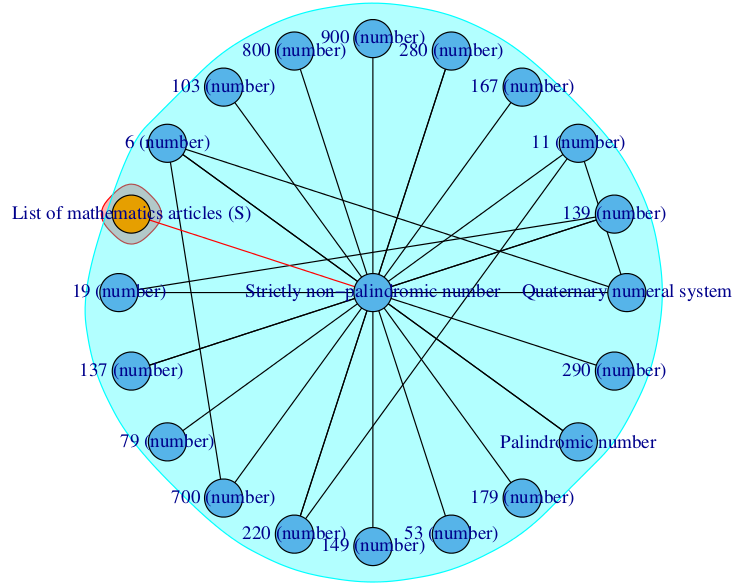
\includegraphics[scale=0.4,keepaspectratio]{Neighbours60}
	\caption{Graph of neighbours of selected vertex and their community membership}
	\label{Neighbours60}
\end{figure}

Fig.~\ref{Neighbours65} perfectly represents situation when the title can be related to more fields. In this example the central vertex \textit{Conjugation} have several meanings in fields such as linguistic, mathematics, biology, chemistry...\footnote{https://en.wikipedia.org/wiki/Conjugation} Most of them are also present in our plot and their division into communities looks reasonable. The green node belongs to linguistics, blue ones to mathematics, and the orange ones to chemistry/biology. This particular case will increase the value of metrics \textit{expansion}, but the division into communities seems logical. This probably happens with all titles that has more than one meaning or are not field specific and therefore could have connection to wide spectrum of other titles. For example almost in every article on Wikipedia we can find some number and therefore make a connection to it -- the question is if it makes sense.

\begin{figure}
	\centering
	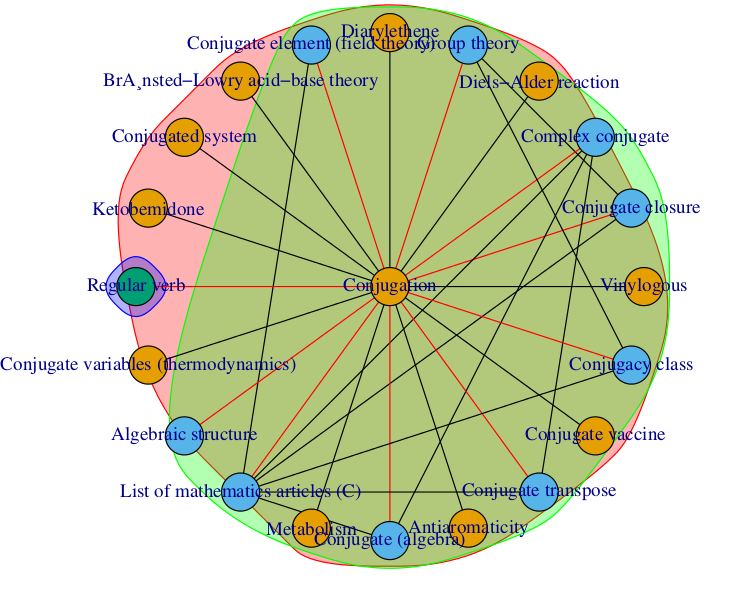
\includegraphics[scale=0.4,keepaspectratio]{Neighbours65}
	\caption{Graph of neighbours of selected vertex and their community membership}
	\label{Neighbours65}
\end{figure}

For most plots of the selected sample that we were able to analyse by this approach division into communities done by fast-greedy algorithm looks like that generally makes sense. 

\subsection{Neighbours in different community}
In this approach we have been looking for the neighbours of each vertex that are not in the same category as the selected vertex. We will look at some examples here, all results can be found in the file \textit{WikiNeighbours.txt} attached to this document.

As with the previous ones, also with this approach we can find situations when division into communities done by fast-greedy algorithm on this data does not get best results. For example, the title \textit{120 (number)} have the neighbour \textit{119 (number)} which is in the different community. This is probably not the result we have expected. But there may be some criteria, which may not be clear just after doing that simple inspection of results, for which keeping these titles in different communities makes sense (for example because of less edges between odd and even numbers). We also cannot assume that the communities are at the same level of generality or specificity when looking at the titles within one community. For example for one community the thing that have all titles in common can by \textit{biology} without possibility to make it more specific, for another it can be \textit{positive numbers divisible by 6}. A lot also depends on the way the links between Wikipedia articles are being made. This process is not uniform for all articles, just because of the way Wikipedia is being made. The same article edited by different people can result, among the other, in different links between articles.

But for the most of the articles we picked to analyse the neighbours in different communities makes sense. For example titles \textit{64 (number)} and \textit{Lowrider} definitely should not be in one category which fast-greedy algorithm recognized well. The question is if the reader of the article about lowriders is interested in knowing more about number 64. 

\subsection{Conclusion}
We have shown that the community detection of this dataset done by fast-greedy algorithm is probably not ideal but generally makes sense. For example it could be used when writing new article to give suggestions for categories to which article belongs (categories can be found down at the end of each article).

We have also discussed some problems with this community detection method on this data. One of them is that process of writing and editing articles at Wikipedia is not uniform and depends by the person that write the article and make connections between articles. Currently the Wikipedia have approximately 50 policies and uses bots to do automated editing of articles\footnote{https://en.wikipedia.org/wiki/Wikipedia}. Therefore there is effort to make the articles in the similar way.

The next fact is that we do not have information when this network have been made, but some links between articles currently cannot be found (for example link to number 64 in the article about lowriders mentioned before). It could be interesting to make same network with the current state of Wikipedia and compare the results.

\section{Appendix}

\end{document}